%% question-16.tex
%%

%% ==============================
\subsection{Diagramme d'objet UML pour le \guillemotleft niveau du sapin\guillemotright}
\label{sec:question15}
%% ==============================

Le code de résolution du niveau présenté à la figure \ref{fig:level}, une fois l'arbre retiré, est  le suivant (Listing \ref{lst:code_level}) :

\begin{figure}
	\centering
	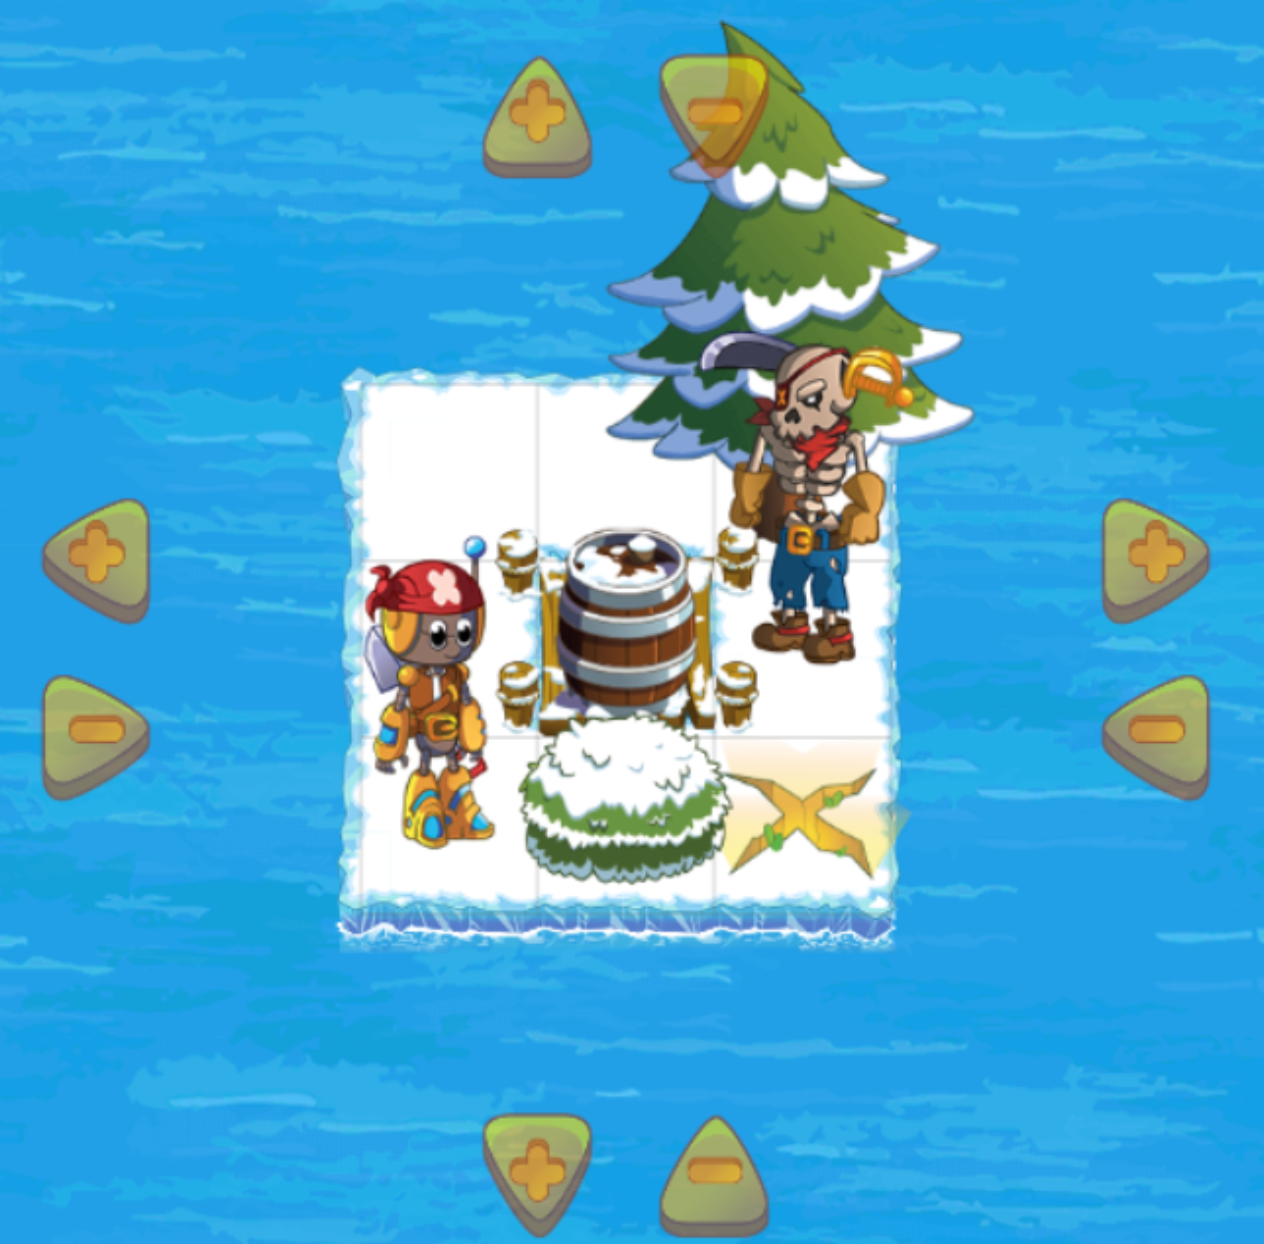
\includegraphics[width=300pt]{assets/level}
	\caption{Le niveau à résoudre}
	\label{fig:level}
\end{figure}

\begin{lstlisting}[caption=Le code permettant de résoudre le niveau,captionpos=b,label={lst:code_level},language=Java]
up(2)
right(2)
/* Permet de changer de direction 
   vers le bas sans se deplacer */
directionDown() 
fight()
down(2)
dig()
\end{lstlisting}

Dans la résolution, nous avons utilisé une instruction d'action \emph{directionDown} qui permet de modifier la direction dans laquelle regarde le joueur sans changer de position. Cela permet de se mettre dans la direction pour frapper l'ennemi.

A partir du code de la solution et de notre diagramme UML, nous pouvons représenter le diagramme d'objet avec la structure présentée ci-après (Figure \ref{fig:diag_obj_1}).

\begin{figure}[h!]
	\centering
	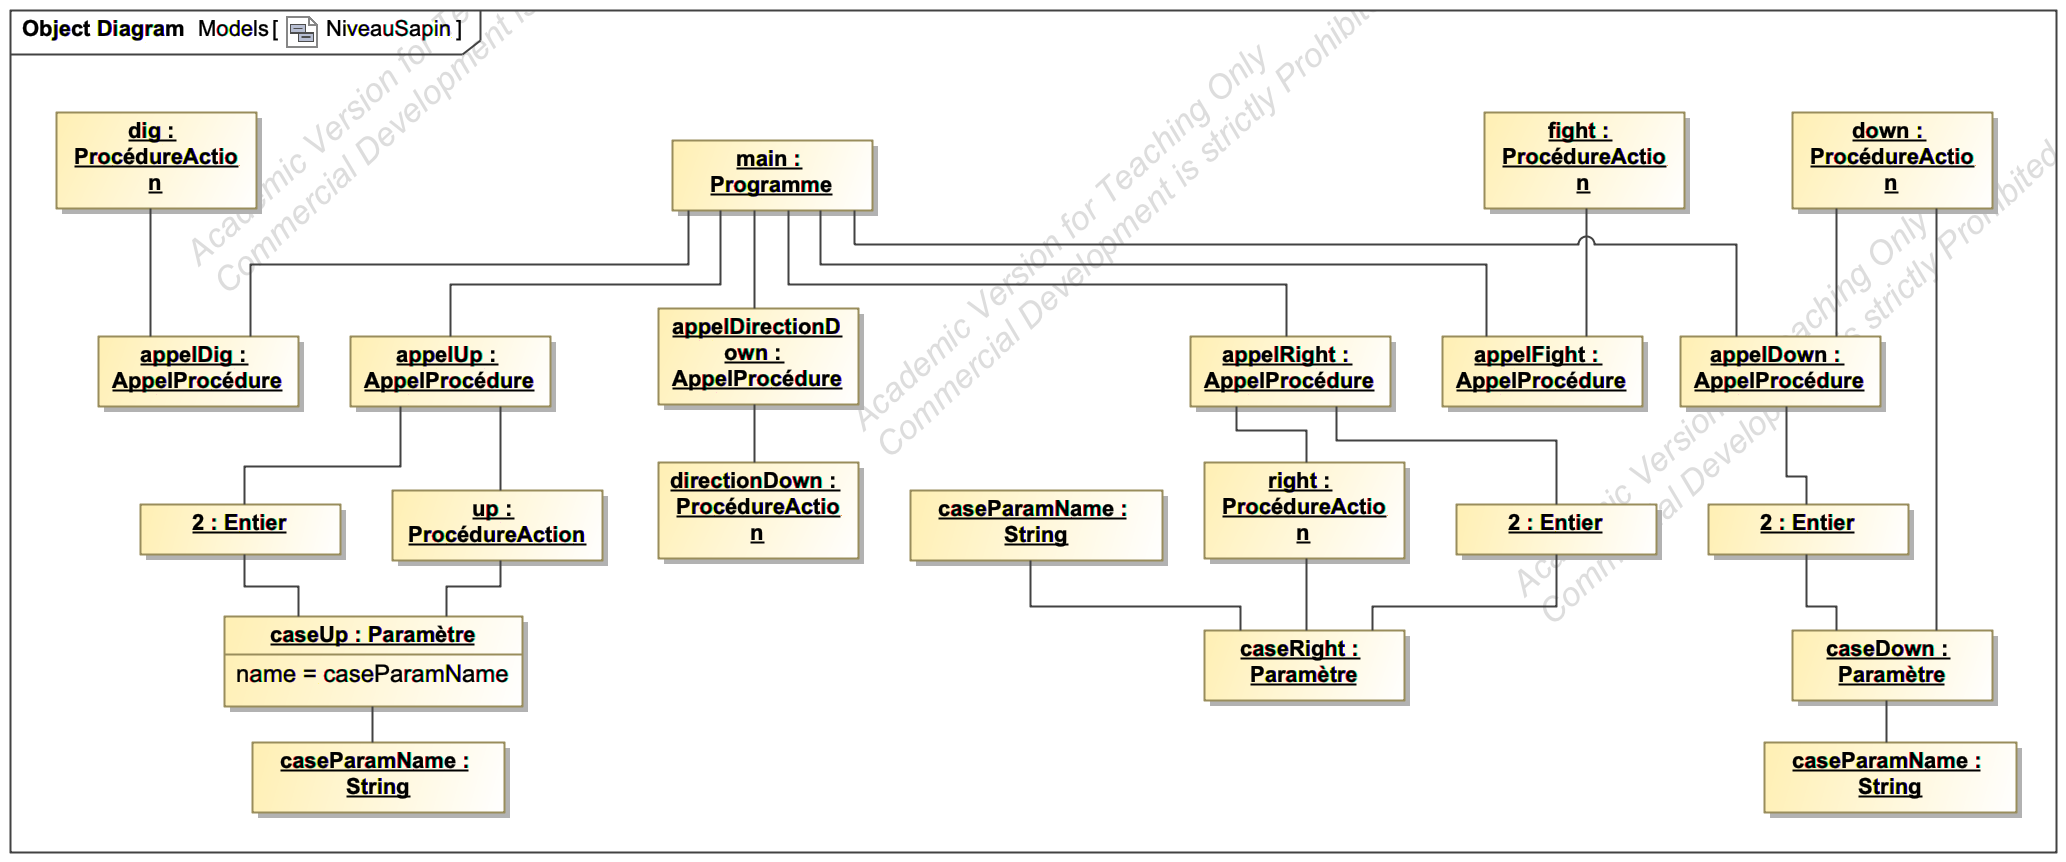
\includegraphics[width=500pt]{assets/obj__NiveauSapin}
	\caption{Diagramme d'objet du programme du niveau du sapin}
	\label{fig:diag_obj_1}
\end{figure}
